\documentclass{beamer}
\usepackage{amsmath}
\usepackage{amssymb}
\usepackage{textpos} % package for the positioning
\usepackage{graphicx} % Allows including images
\usepackage{tikz} % for those who hate themselves
\usetikzlibrary{calc}
\usepackage{mwe}
\usetikzlibrary{positioning}

\mode<presentation>{
\usetheme{Rochester}

\setbeamertemplate{navigation symbols}{} % To remove the navigation symbols from the bottom of all slides uncomment this line

\definecolor{OUGold}{RGB}{181,154,57}
\setbeamercolor{structure}{fg=OUGold}
\setbeamercolor{block title example}{bg=OUGold}
\setbeamercolor{section in toc}{fg=black}

% position the logo
\addtobeamertemplate{frametitle}{}{
	\begin{textblock*}{\paperwidth}(290pt,-38pt)
		
\includegraphics[height=1cm,keepaspectratio]{sail}
\end{textblock*}}
}



\title[Adaptive Sampling of Cardiac Action Potentials]{Adaptive Sampling of Cardiac Action Potentials for a Best Fit Ellipse}
\author[Medcoff]{Jason Medcoff}
\institute{
	        Oakland University
}
\date{Meeting of Minds, 11 May 2018}

\begin{document}
	
	\begin{frame}
		\frametitle{\space}
		\titlepage
	\end{frame}
	
	\begin{frame}
		\frametitle{Motivation}
		\begin{itemize}
			\item Fibrillation and treatment: large electric shocks
			\item Drug therapies don't work! (Pratt and Moye, 1995)
			\item Another idea: do more with less
		\end{itemize}
	$\newline$
	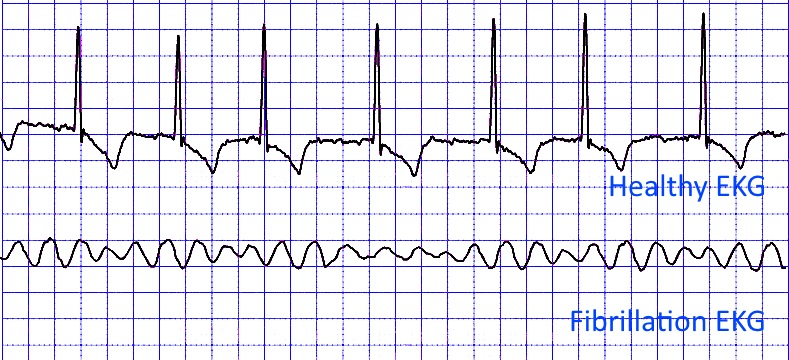
\includegraphics[scale=0.5]{ekg.jpg}
	
	\end{frame}

	\begin{frame}
		\frametitle{Motivation}
		\begin{itemize}
			\item Small electric shocks instead of one big one
			\item more understanding as a math/physics problem (since math is easier than biology)
			
		\end{itemize}
	\begin{center}
		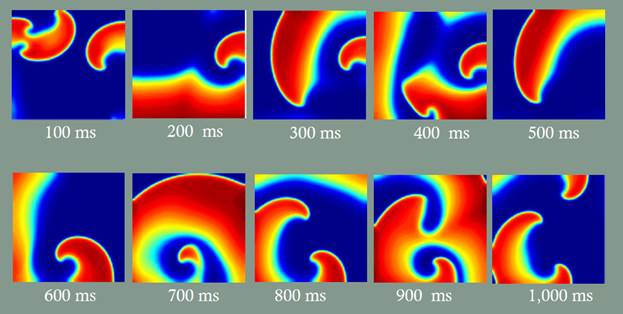
\includegraphics[scale=0.5]{spiral.jpg}
	\end{center}
	\end{frame}
	
	

	\begin{frame}
		\frametitle{The model}
		Fenton et. al., 2002
		$$ \frac{\partial V_m}{\partial t} = D \nabla^2 V_m - \frac{I_{ion}+I_{stim}}{C_m} $$
		$$ I_{fi} = \frac{-\nu p(V_m - V_c)(1-V_m)}{\tau_d} $$
		$$ I_{so} = \frac{V_m (1-p)}{\tau_0} + \frac{p}{\tau_r} $$
		$$ I_{si} \frac{-w(1+\tanh(k(V_m-V_c^{si})))}{2\tau_{si}} $$
		$I_{fi}$: sodium upstroke \\
		$I_{si}$: calcium plateau \\
		$I_{so}$: potassium downstroke \\
		$I_{stim}$: stimulus current (experiment)
	\end{frame}

	
	\begin{frame}
		\frametitle{And when we do this...}
		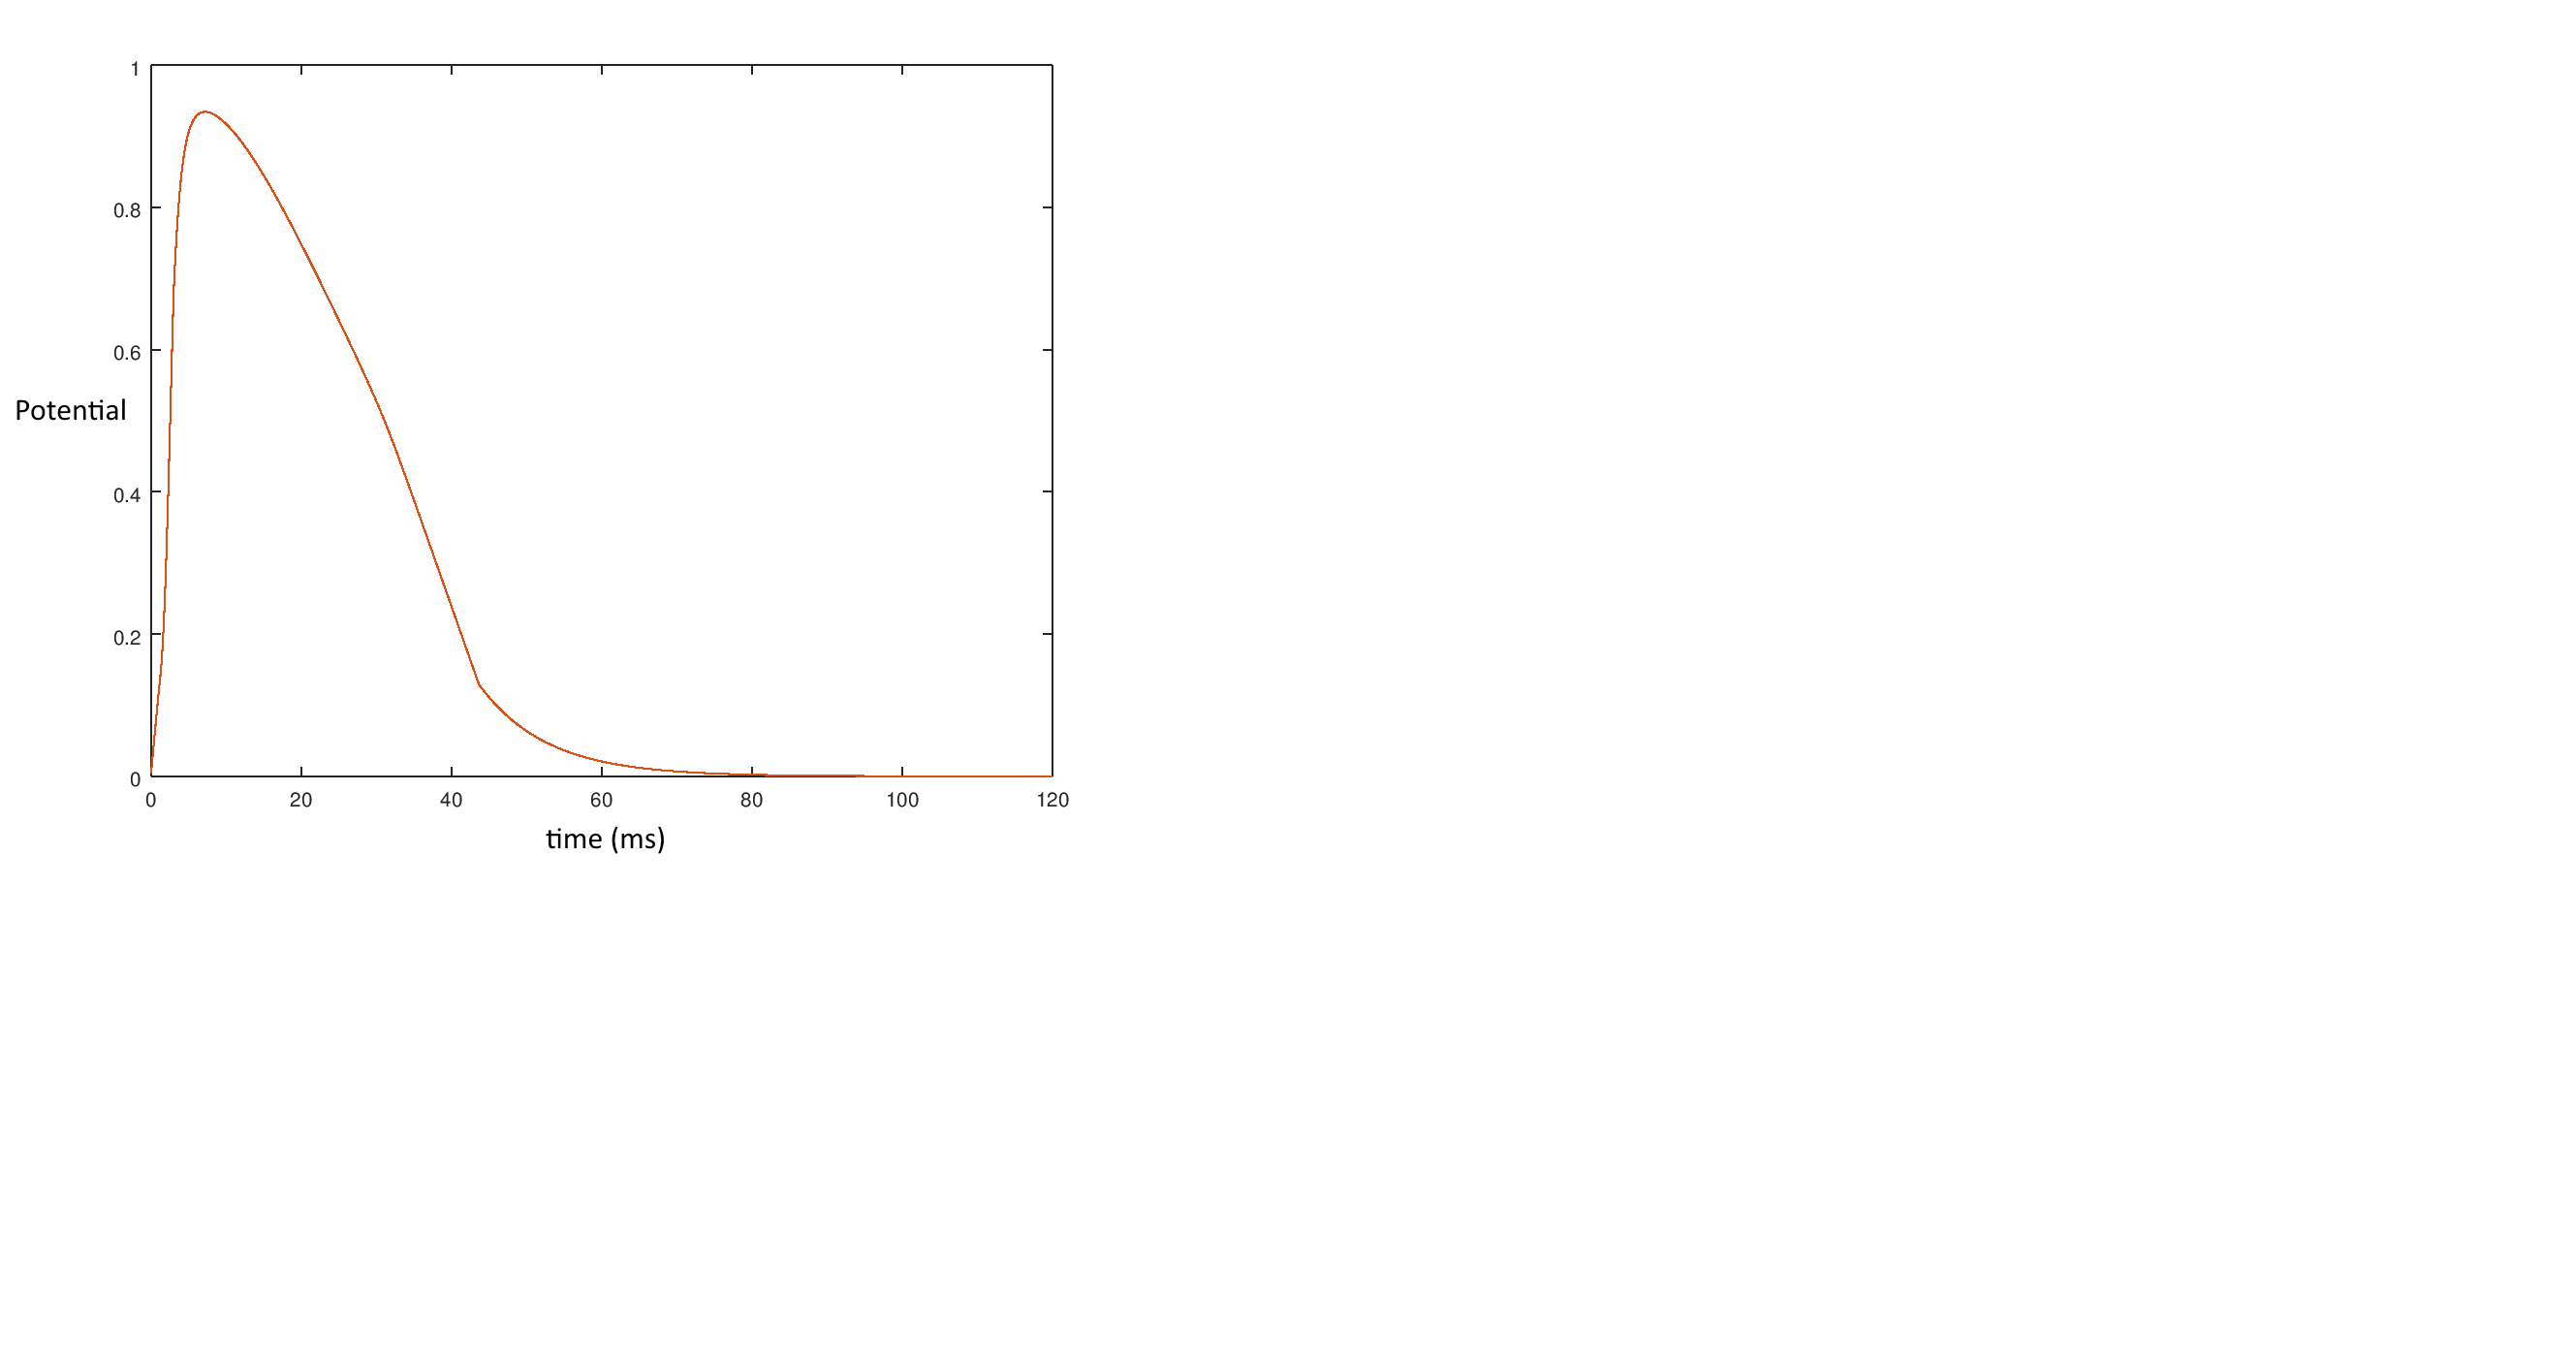
\includegraphics[scale=0.5]{ap.png}

	\end{frame}

	\begin{frame}
		\frametitle{Phase space}
		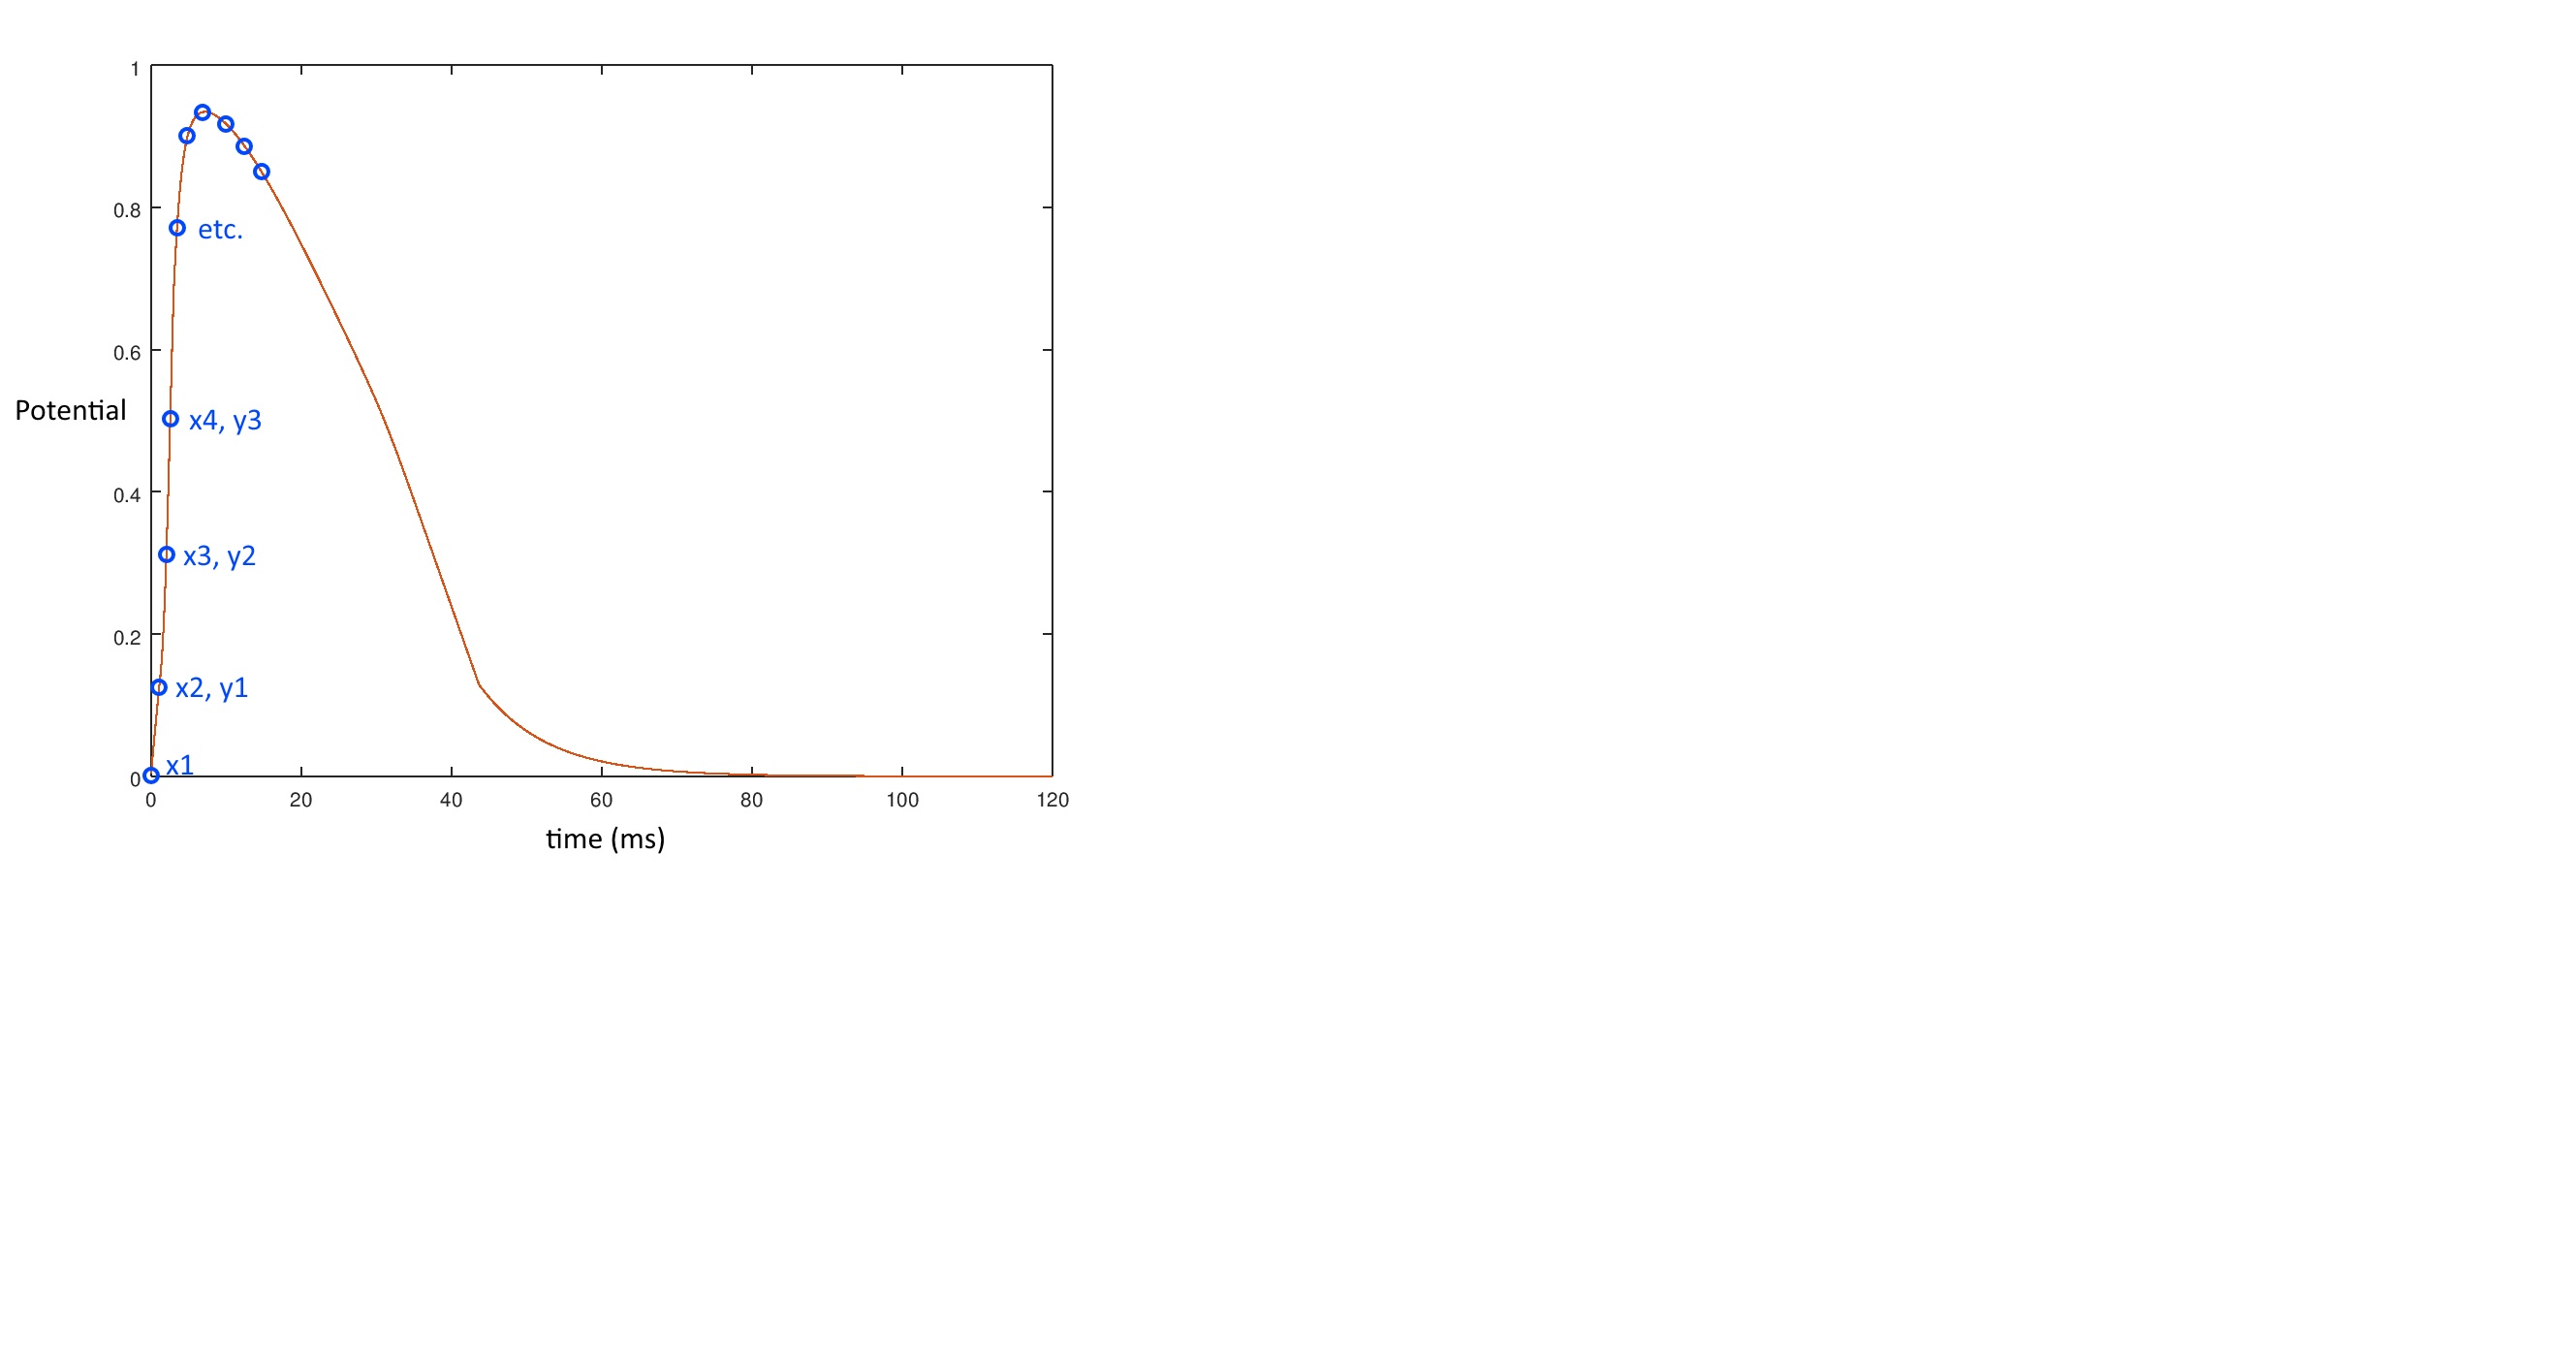
\includegraphics[scale=0.5]{phase.jpg}
	\end{frame}

	\begin{frame}
		\frametitle{The model}
		\begin{itemize}
			\item Back away from the biology, what's happening?
			\item a toroidal attractor in phase space
			$\newline \newline$
		\end{itemize}
		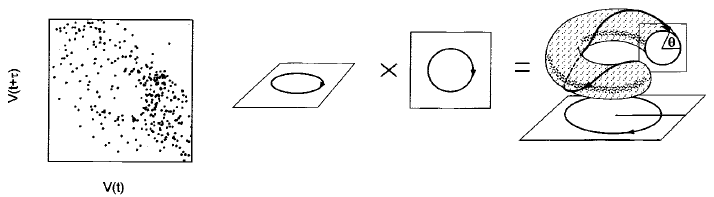
\includegraphics[scale=0.4]{torus.png}
	\end{frame}
	
	\begin{frame}
		\frametitle{Method}
		\begin{itemize}
			\item The idea: sample discrete points on this signal
			\item plot into phase space as $V(t)$ against $V(t+\Delta t)$
			\item important consideration: choosing $\Delta t$
			\item cater to experimentalists!
		\end{itemize}
	\end{frame}

	\begin{frame}
		\frametitle{Method}
		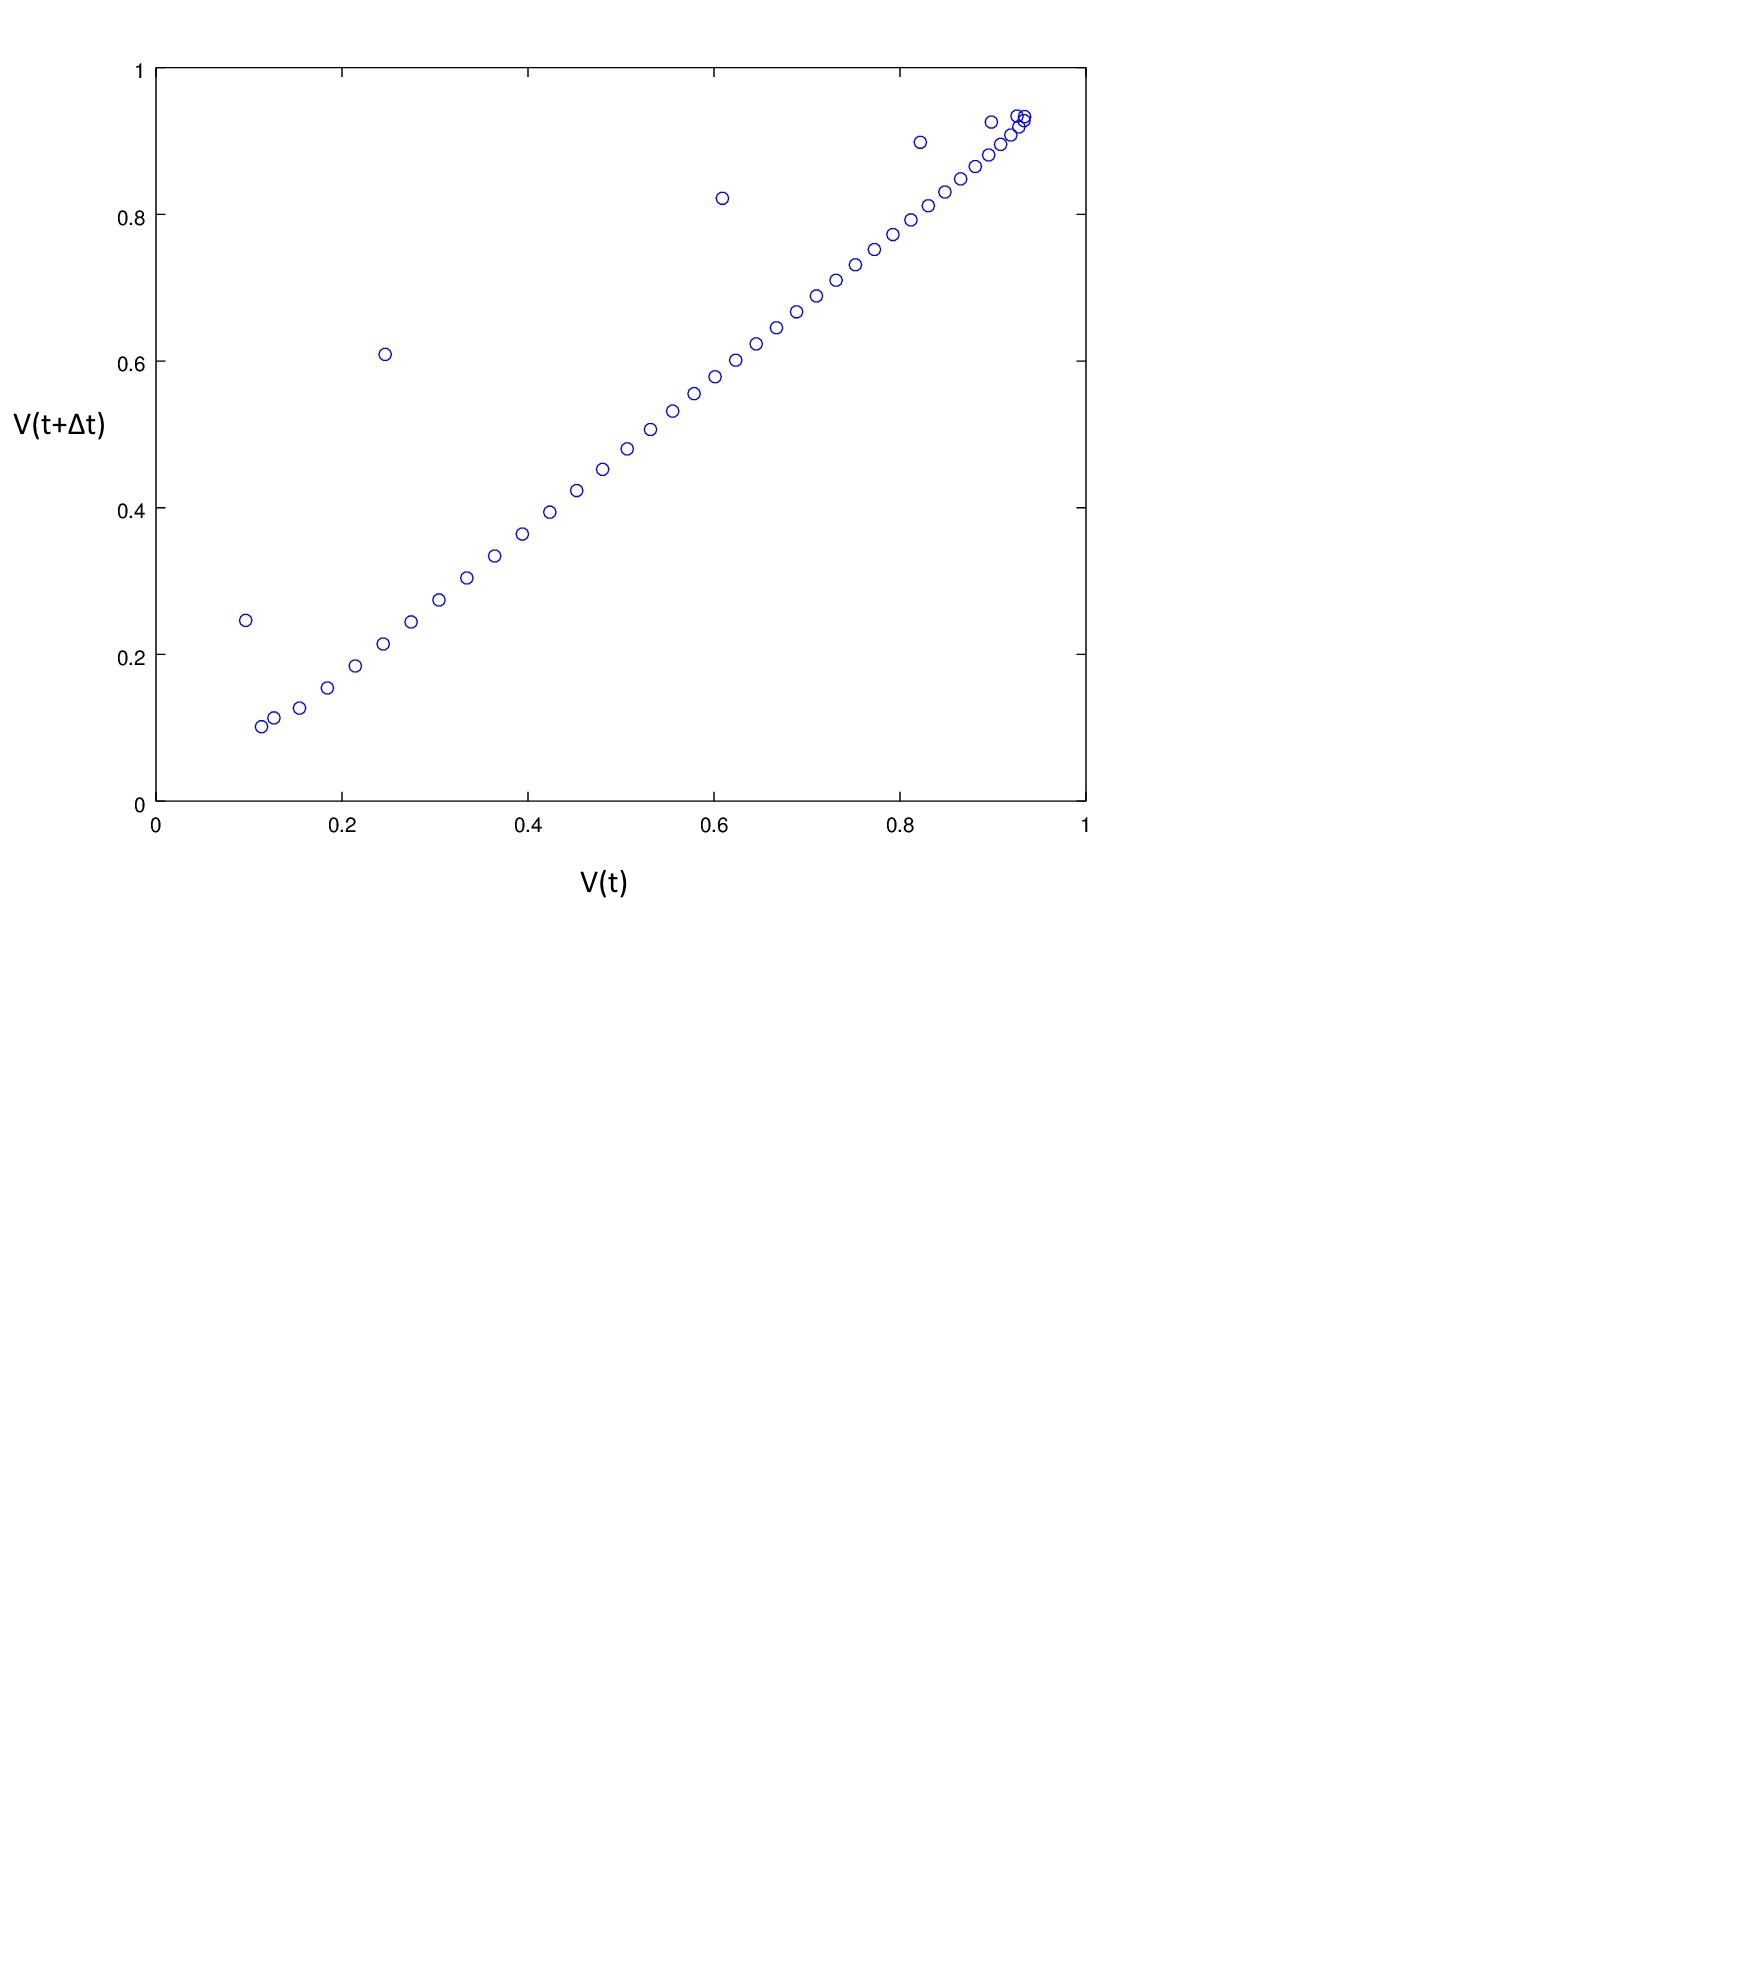
\includegraphics[scale=0.5]{normalsampling.jpg}
	\end{frame}

	\begin{frame}
		\frametitle{Issues}
		What happens when we try to fit an ellipse?
		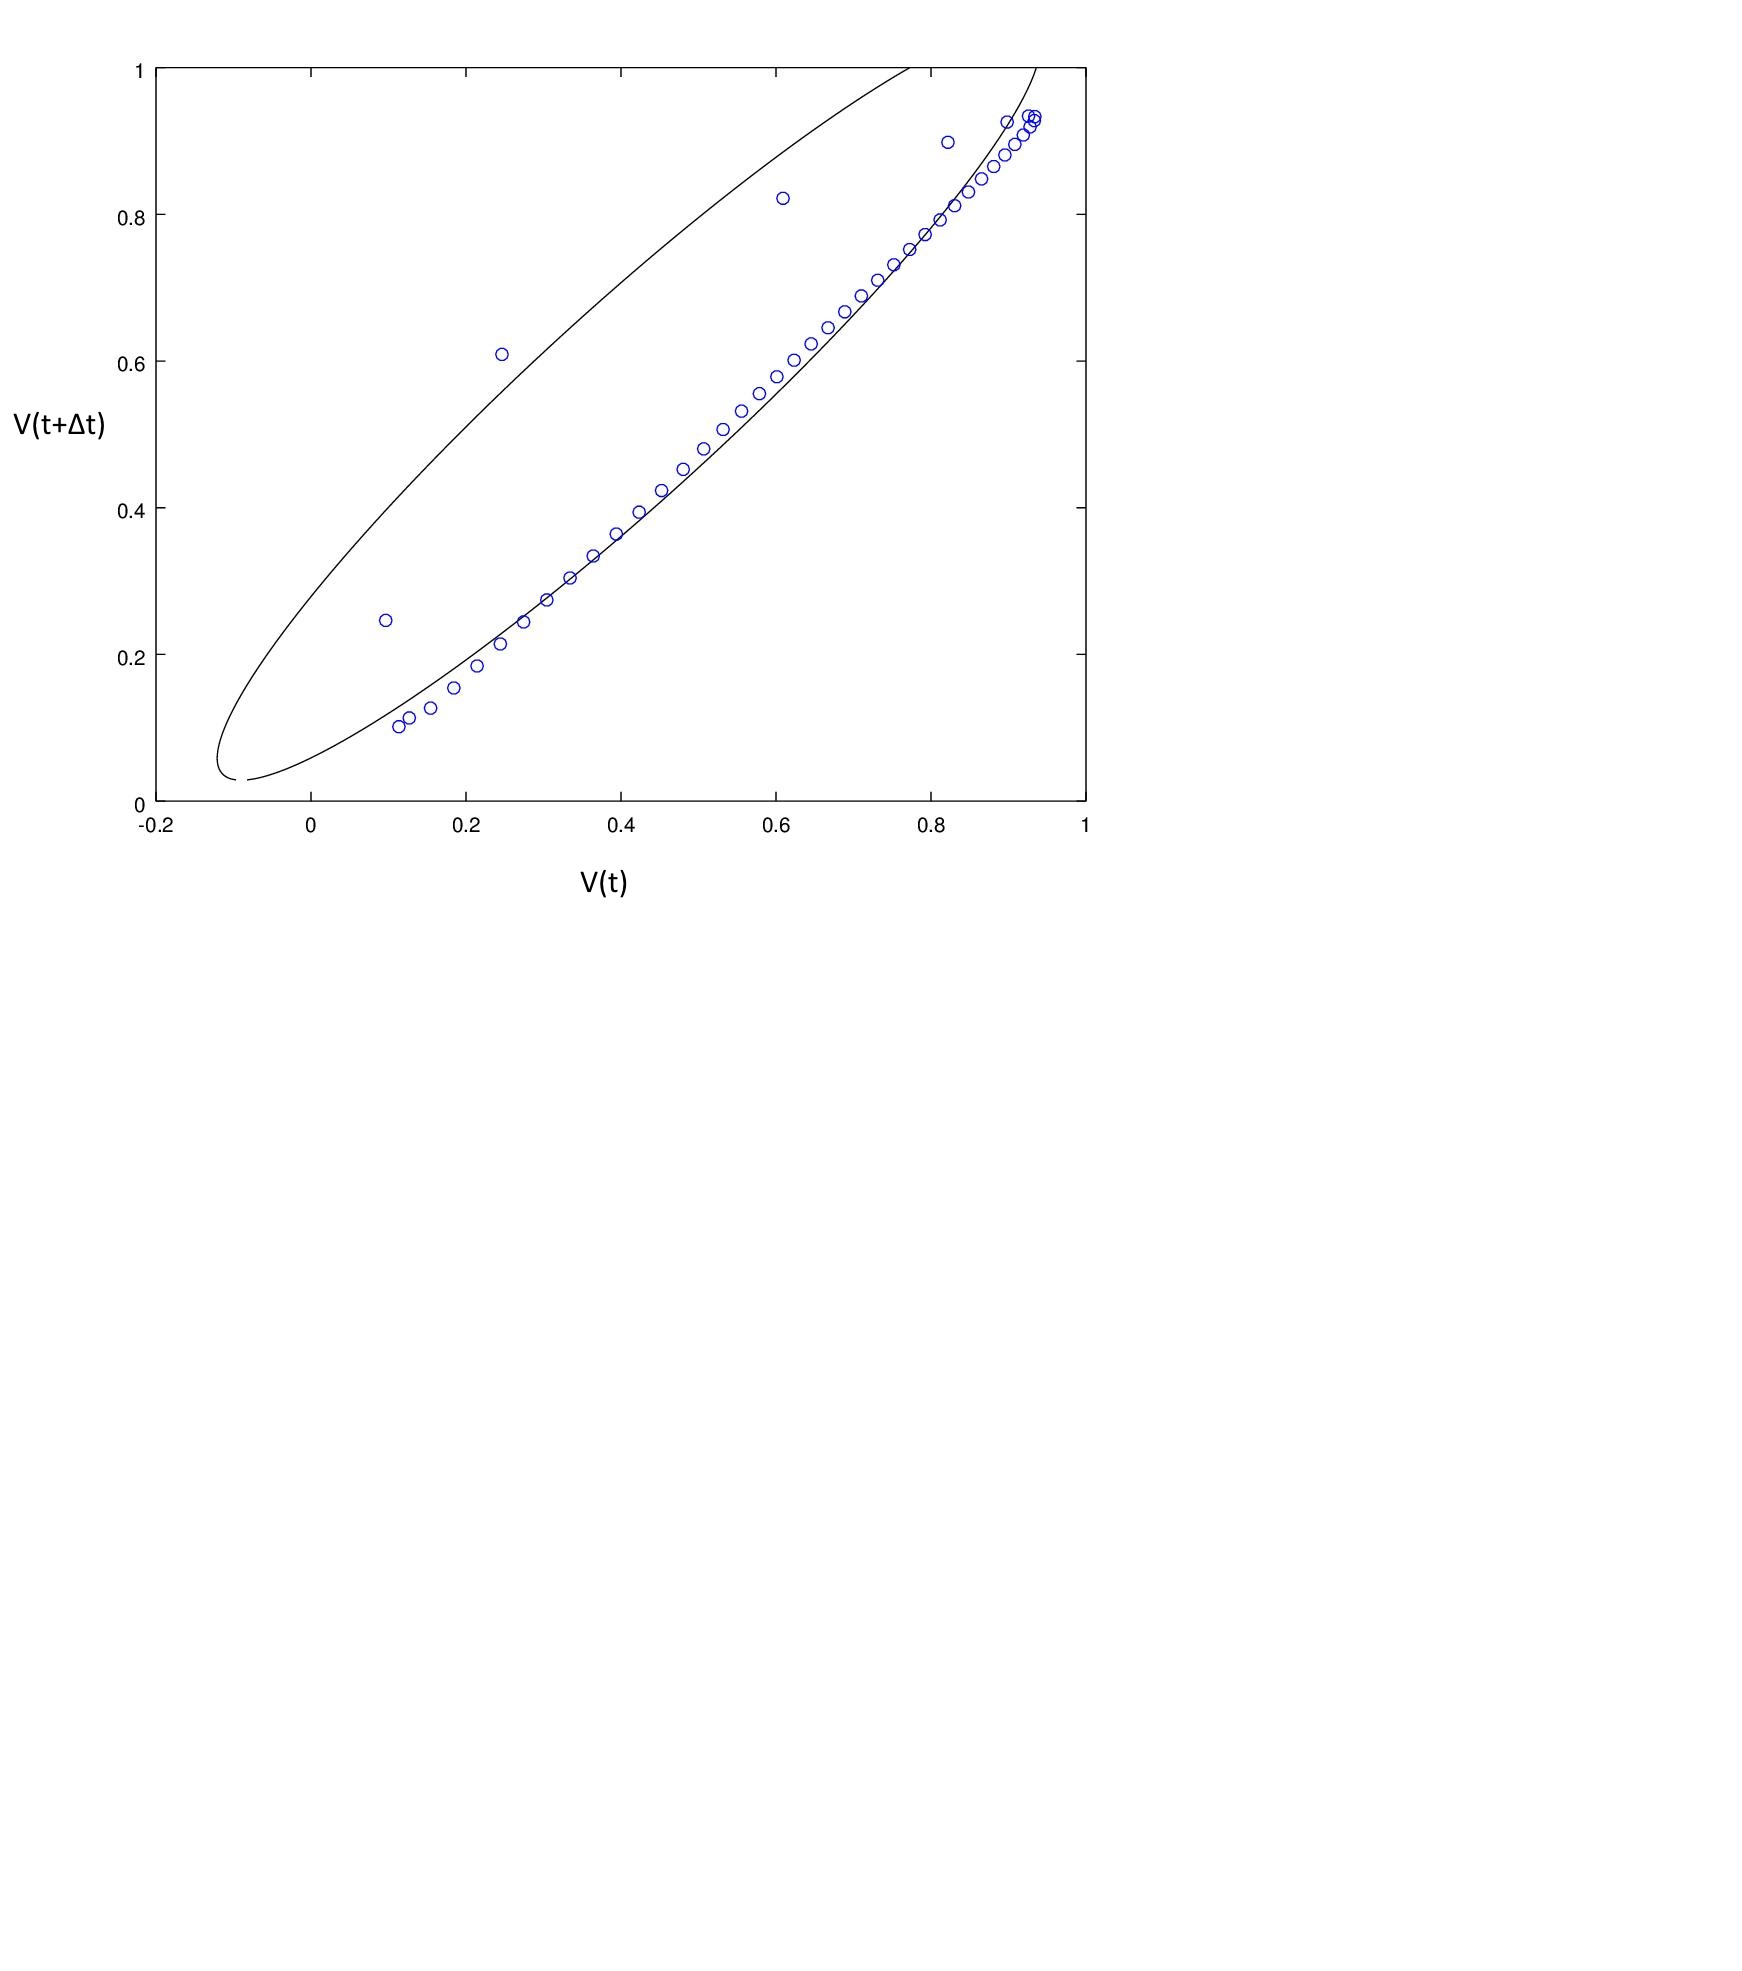
\includegraphics[scale=0.45]{normalellipse.jpg}
	\end{frame}
	
	\begin{frame}
		\frametitle{Issues}
		\begin{itemize}
			\item to the computer's eyes, perfectly fine
			\item to a human's eyes, not so much
			\item the issue: point density
		\end{itemize}
	\end{frame}
	
	\begin{frame}
		\frametitle{New method}
		\begin{itemize}
			\item What if we relax the conditions on $\Delta t$?
			\item Say, for an action potential of length $N$ with upstroke duration $n$, we choose $\Delta t = \frac{n}{N}$ during the upstroke
			\item How does this compare to the old method?
		\end{itemize}
	\end{frame}
	
	\begin{frame}
		\frametitle{New method}
		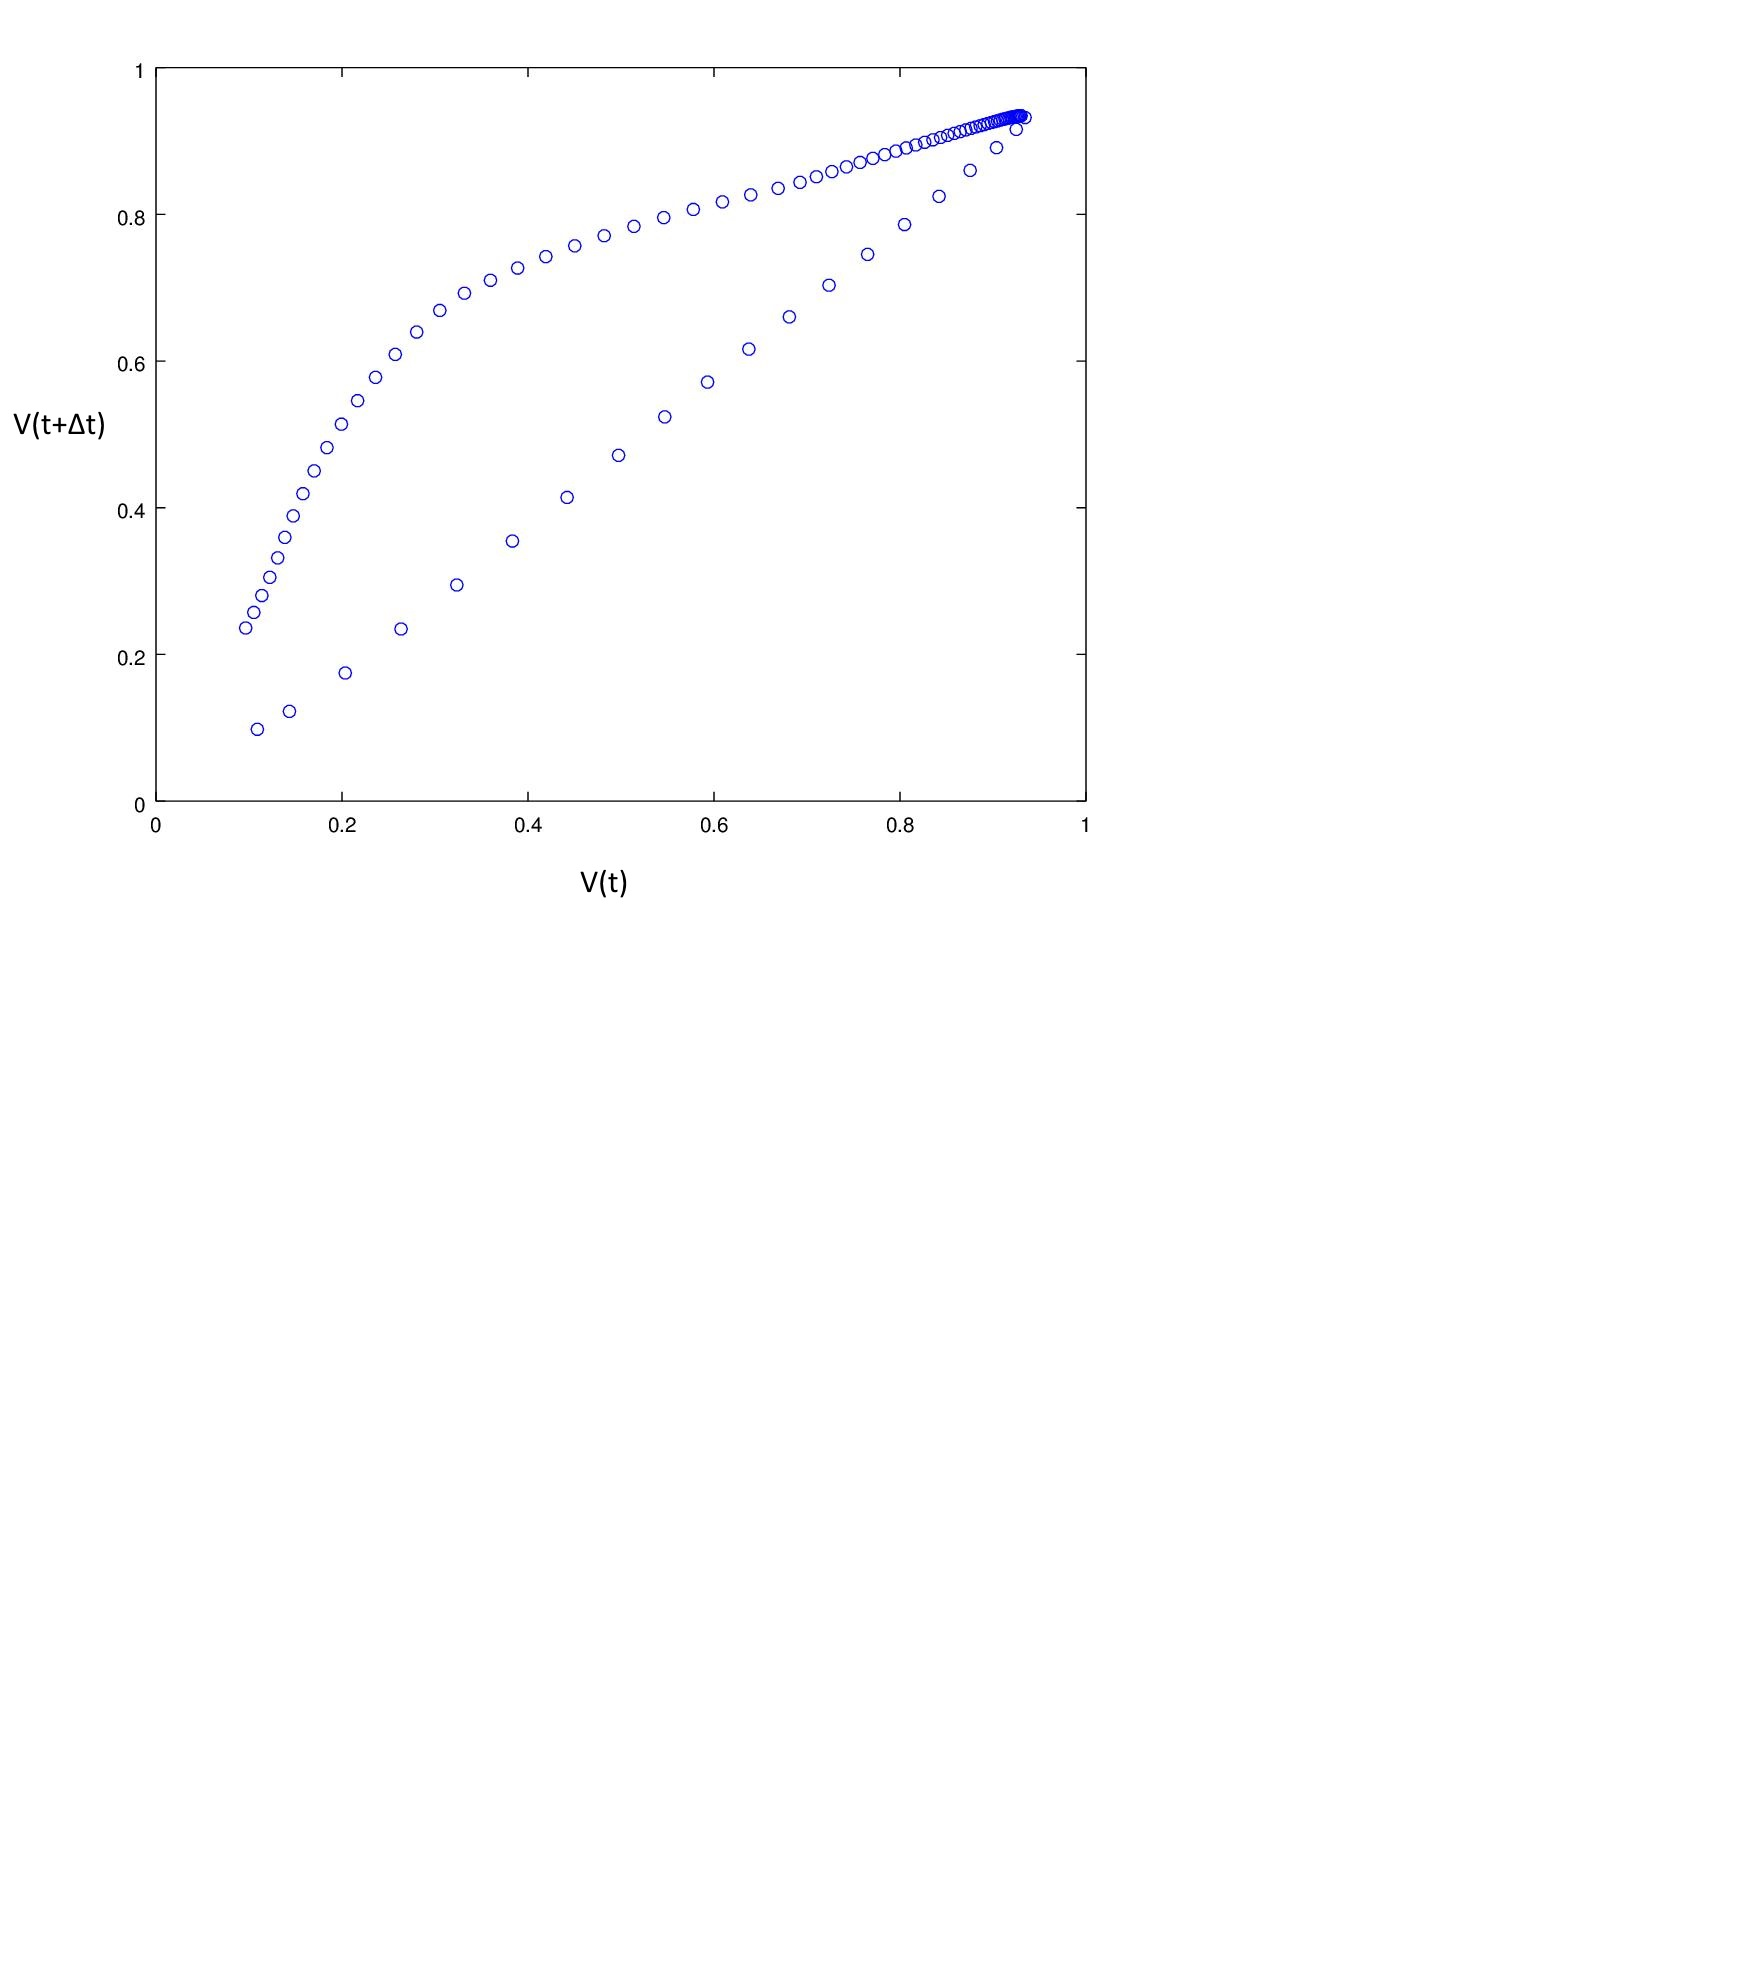
\includegraphics[scale=0.5]{adaptivesampling.jpg}
	\end{frame}
	
	\begin{frame}
		\frametitle{New Method}
		Better?
		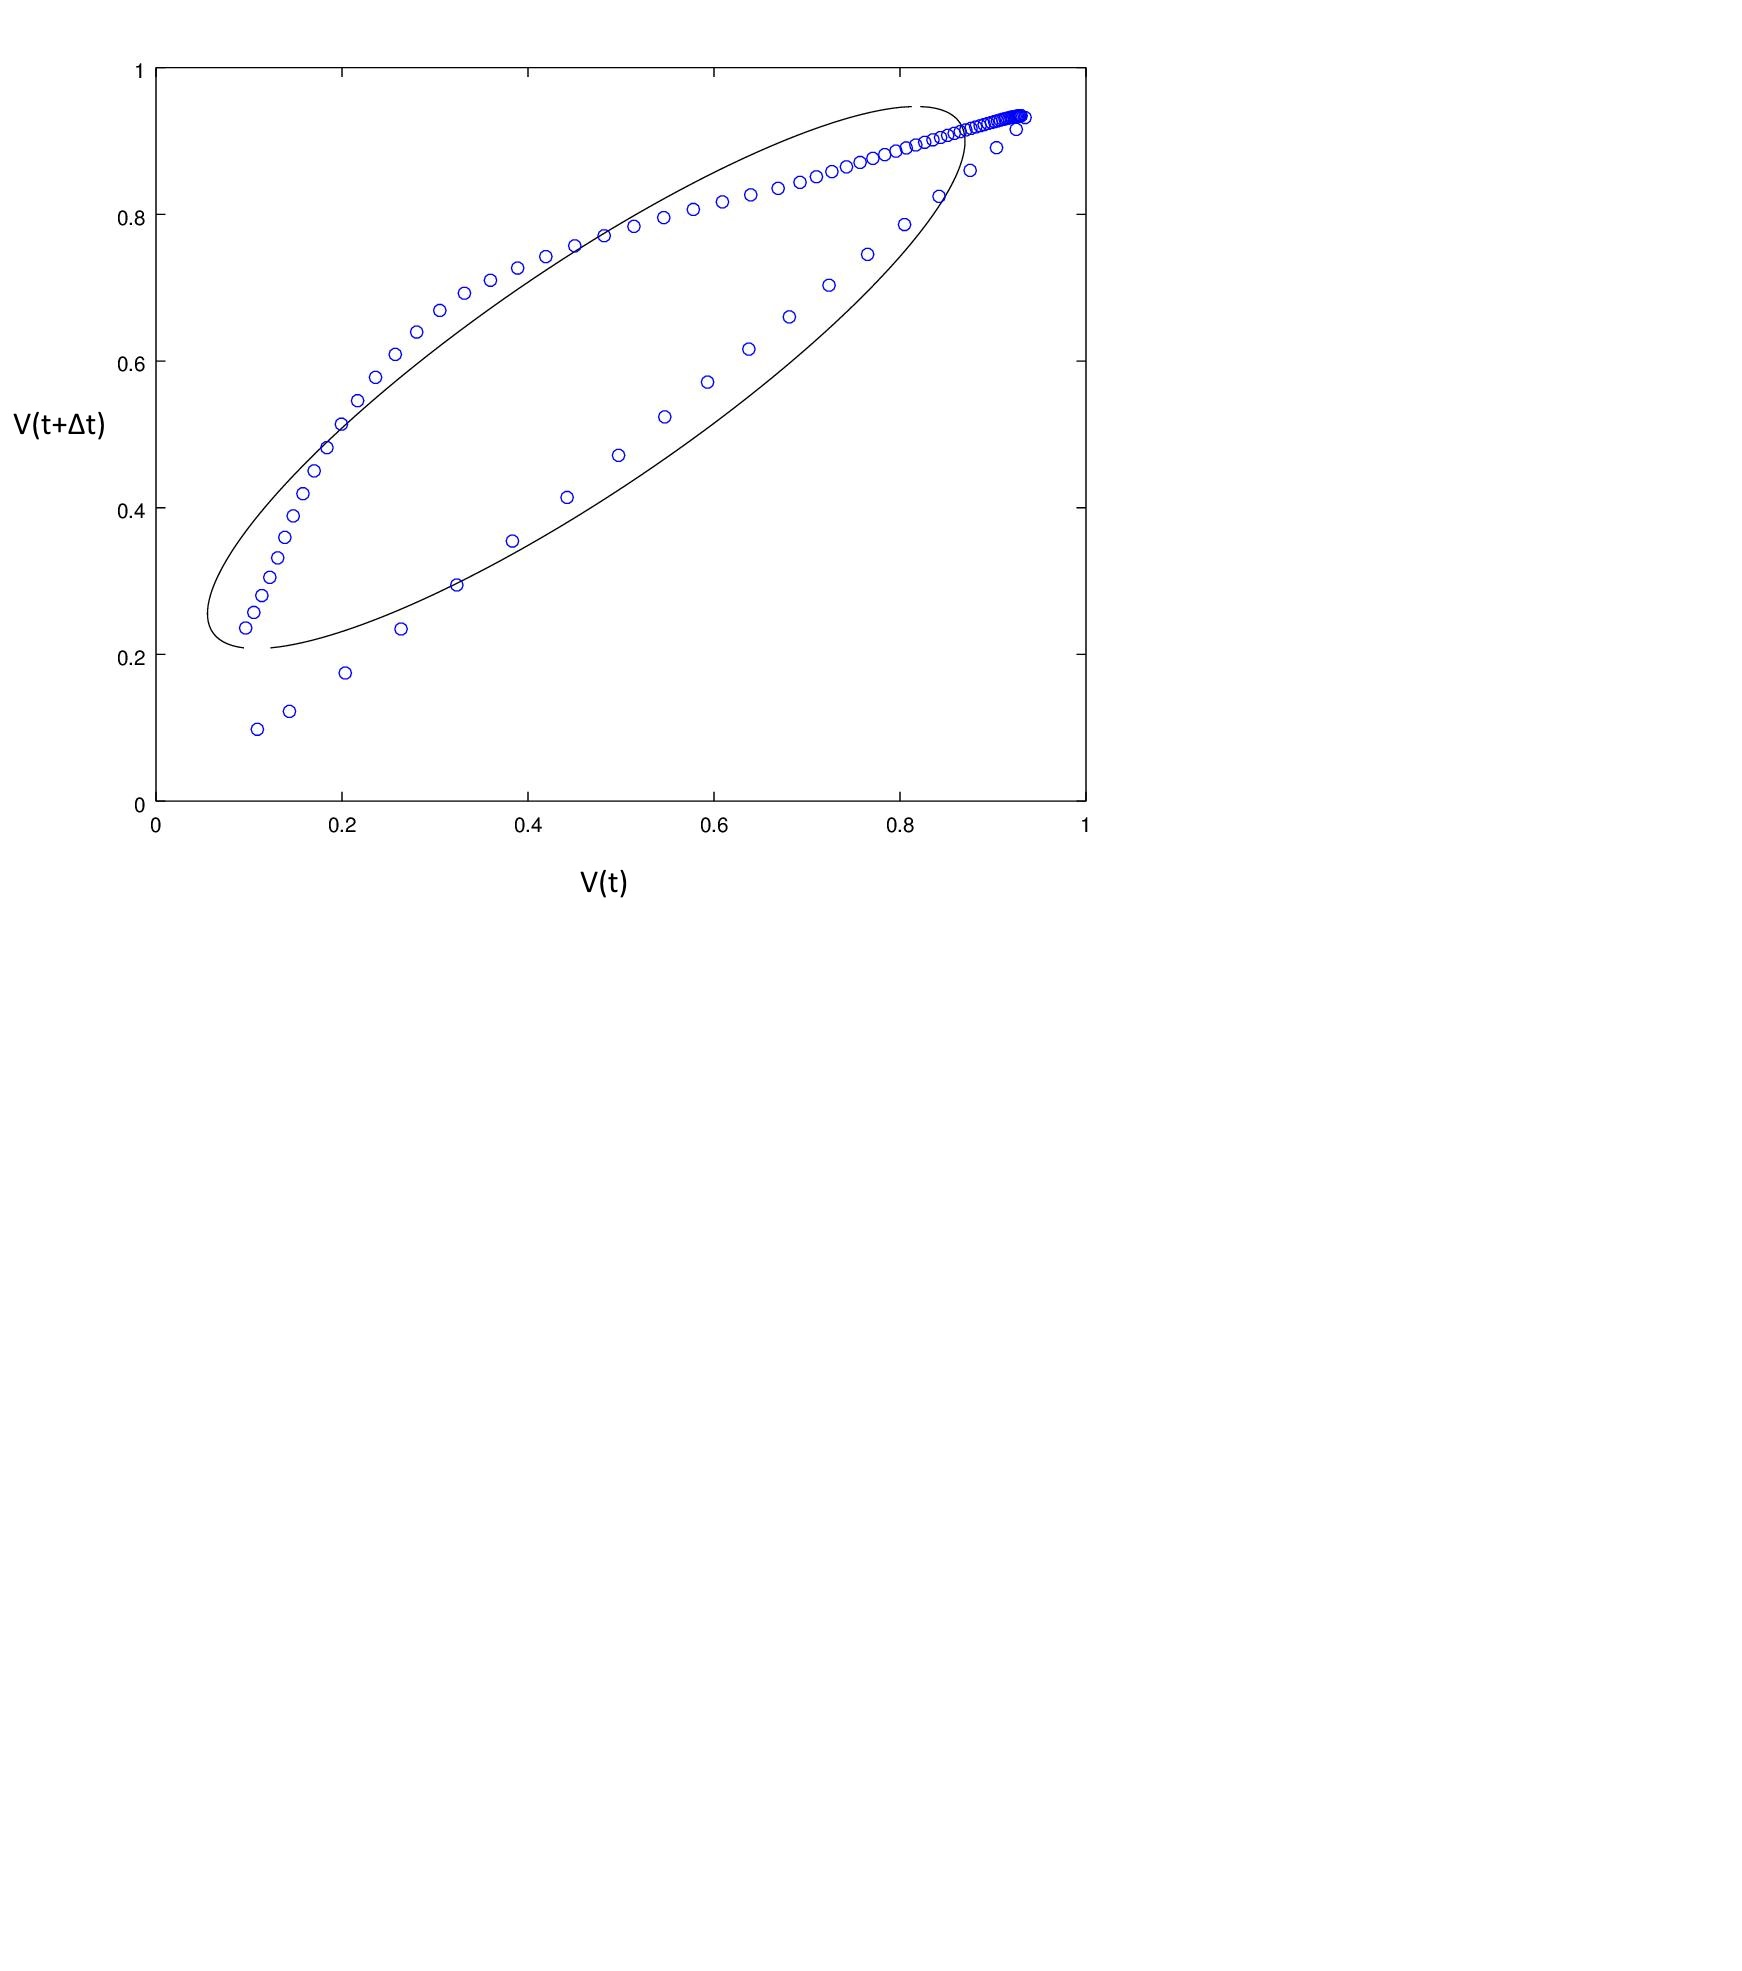
\includegraphics[scale=0.45]{adaptiveellipse.jpg}
		
	\end{frame}

	\begin{frame}
		\frametitle{An application}
		\begin{itemize}
			\item using this method to explore correlations in drug therapy
			\item dotted: eccentricity, dashed/dot-dashed: semimajor/minor axes, solid: termination of fibrillation 
		\end{itemize}
	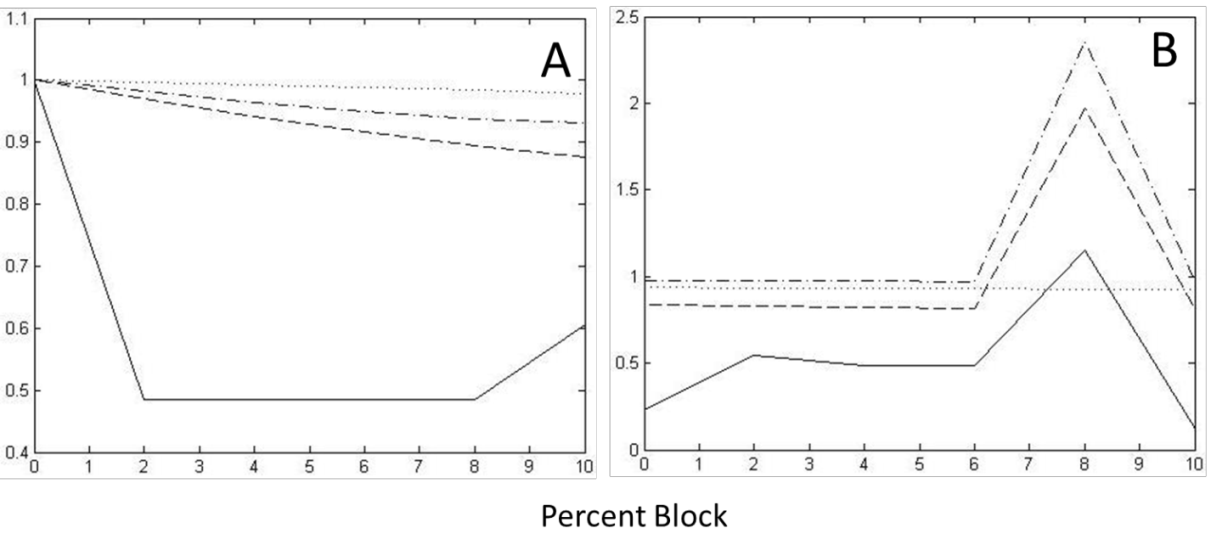
\includegraphics[scale=0.25]{data.png}
		
	\end{frame}

	\begin{frame}
		\frametitle{Summary}
		\begin{itemize}
			\item make a geometric connection to raw data: represent phase space trajectories by ellipses
			\item interpret the data such that the geometry makes sense: choose $\Delta t$ appropriately
			\item use the geometry to observe correlations: measure eccentricity, axis length, etc.
		\end{itemize}
	\end{frame}

	\begin{frame}
		\frametitle{Future work}
		\begin{itemize}
			\item How should we choose the sampling ratio?
			\begin{itemize}
				\item static ratio based on length of upstroke?
				\item dynamic ratio based on some metric in phase space?
			\end{itemize}
			\item How many points do we need to work with?
			\item Application: do the best-fit ellipses provide a reliable descriptor of fibrillation termination rates? (big for the experimentalists)
		\end{itemize}
	
	\end{frame}

	\begin{frame}
		\frametitle{Acknowledgements}
		\begin{itemize}
			\item Grace Goodrich, Shelby Gulda, Alyson Light, Sharon Taragaturi
			\item Dr.\ Brad Roth
			\item Dr.\ Steffan Puwal
		\end{itemize}
	\end{frame}

	
\end{document}